% !TEX encoding = UTF-8 Unicode
% !TEX root = project.tex

\section{Evaluation}
\label{sec:finding}

In order to evaluate the effectiveness of our tool, we ran experiments on existing projects in GitHub. We created an evaluation version of this tool that would fetch related files based on only the files from the first commit of a pull request. Normally, our tool gathers related files from the latest set of items in a given pull request, taking into account all of the latest commits. However, we wanted to know the files that would be related from the first commit so that we can compare the results against what was subsequently committed afterwards. This comparison would give us an idea of how helpful our tool would have been had the developers used it after their first commit. From the small sample set of data that we evaluated against, we found that of the 87 total new files that were added after the first commit, 17 (19.5\%) of new files were found to be related by our tool.

\subsection{Evaluation Setup}

We gathered data from 5 projects in GitHub: videojs~\cite{videojs}, moviepy~\cite{moviepy}, cocos2d-x~\cite{cocos2d-x}, OpenRA~\cite{OpenRA}, and jmonkey~\cite{jmonkey}. The project descriptions and their associated languages are listed in Table \ref{tab:evaluationprojects} below. 

\begin{table}[h]
\centering
\begin{tabular}{lll}
\hline
Project & Description & Language \\
\hline
videojs & Video player & Javascript \\
moviepy & Video editor & Python \\
cocos2d-x & 2D game engine & C++ \\
OpenRA & Game engine & C\# \\
jmonkey & 3D game engine & Java \\
\hline
\end{tabular}
\caption{Projects used for evaluation.}
\label{tab:evaluationprojects}
\end{table}

All of these open source GitHub projects have several contributors. As such, this will reduce the possibility of attaining any conclusions based on any peculiar development behaviors from any single developer. All of the projects differ in programming languages as well. From the 5 projects, we explored a total of 329 pull requests looking for cases where the pull requests had: 

\begin{itemize}
  \item multiple commits; and
  \item subsequent commits added at least one additional file.
\end{itemize}

We found 29 such pull requests that matched this criteria. Given the short amount of time for this project, we decided that this sample set was sufficient for our purposes.

\subsection{Evaluation Results}

With the 29 pull requests that matched our evaluation criteria, we used the evaluation version of our tool to find the related files from the first commit. Once we had the related files, we compared the resulting files with the final set of files that were committed in the pull request. Figure \ref{fig:committedAndRelatedFiles} shows the breakdown of the number of files from the first commit, the new files added after the first commit, and the number of recommended files across all 5 projects. For all projects except for OpenRA, the number of recommended files were greater than the number of new files added. Also, the OpenRA and cocos2d-x projects contributed the most with regard to the amount of data collected as these projects are more mature with several candidate pull requests that we were able to use.

\begin{figure}[h!]
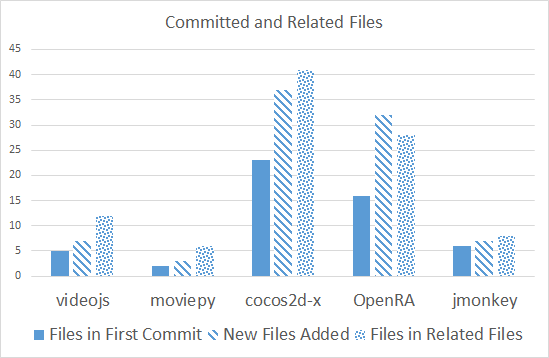
\includegraphics[width=8cm]{CommittedAndRelatedFiles}
\caption{Comparison of the number of files after the first commit, new files added afterwards, and files that were recommended in the 'Related Files' tab based on the files from the first commit.}
\label{fig:committedAndRelatedFiles}
\end{figure}

Figure \ref{fig:newFilesAfterFirstCommit} displays the number of new files that were added after the first commit. This figure further breaks down whether these new files were recommended by our tool or not. From this data, a total of 87 new files were added from the 29 pull requests that we explored. Of the 87 new files, 17 files were recommended by our tool. With the small sample set that we worked with, this gives us a general idea that 19.5\% of new files added may be recommended with the tool. This is an interesting result as it loosely claims that 1 in 5 new files added after the first commit may be recommended by our tool. This may help developers ensure that they are not missing any related files when they make changes to existing code.

\begin{figure}[h!]
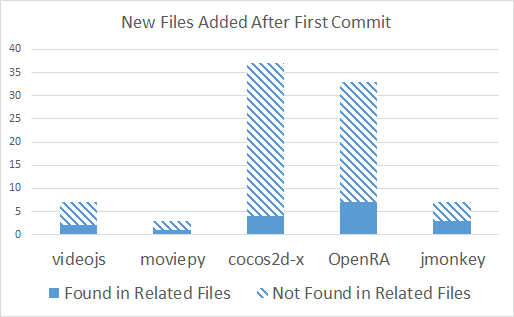
\includegraphics[width=8cm]{NewFilesAfterFirstCommit}
\caption{Comparison of the new files added after the first commit that were recommended in the 'Related Files' tab.}
\label{fig:newFilesAfterFirstCommit}
\end{figure}

\subsection{Threats to Validity}

\subsubsection{Small Sample Set}

The sample size of pull requests that we used for evaluation is quite small. We were limited to manually inspect the pull requests for candidate matches rather than writing a tool to mine this data automatically. This limitation was due to the short amount of time that we had for this project. Future work may include authoring a tool that would effectively mine this data from GitHub and verify the usefulness of our tool in a more proficient manner. Also, even though we gathered data from 5 different projects, we are not claiming that this data is representative of all types of software projects. The 5 projects differ in programming languages but they are similar in that 2 are video related projects and the other 3 are game engine projects. With a larger sample set of test data that spans several more projects, we would be able to get a better idea of the effectiveness of our tool.

\subsubsection{Developer Behaviors}

All developers are different and with that, most developers have different behaviors. Related to the small sample set limitation described above, we cannot avoid the possibility of using data where the developer behaved in an abnormal manner. For instance, it is completely possible that a developer may commit the first set of files with the intention of continuing and adding files at a future date. In this sense, the developer knows that they will commit more files later or even in another pull request. Our tool does not take this behavior into account as it solely looks at the files in a single pull request.

\subsubsection{Types of Changes Made}

From exploring hundreds of pull requests, we have noticed that there are several types of software changes that are made where our tool may be more applicable. Generally, for changes that are made where the modifications are in a focused area of a system where few components are affected, such as a small bug fix or a small newly added feature, our tool is most effective. However, for changes that span a wide area of seemingly unrelated components, such as general comment additions, or spelling corrections, it is difficult for our tool to adequately recommend associated files as the changes may not be functionally related to each other.